% !TEX root = ../main.tex
\section{Satoshi HBO Market}
\label{app:hbo}

\begin{figure}
  \centering
  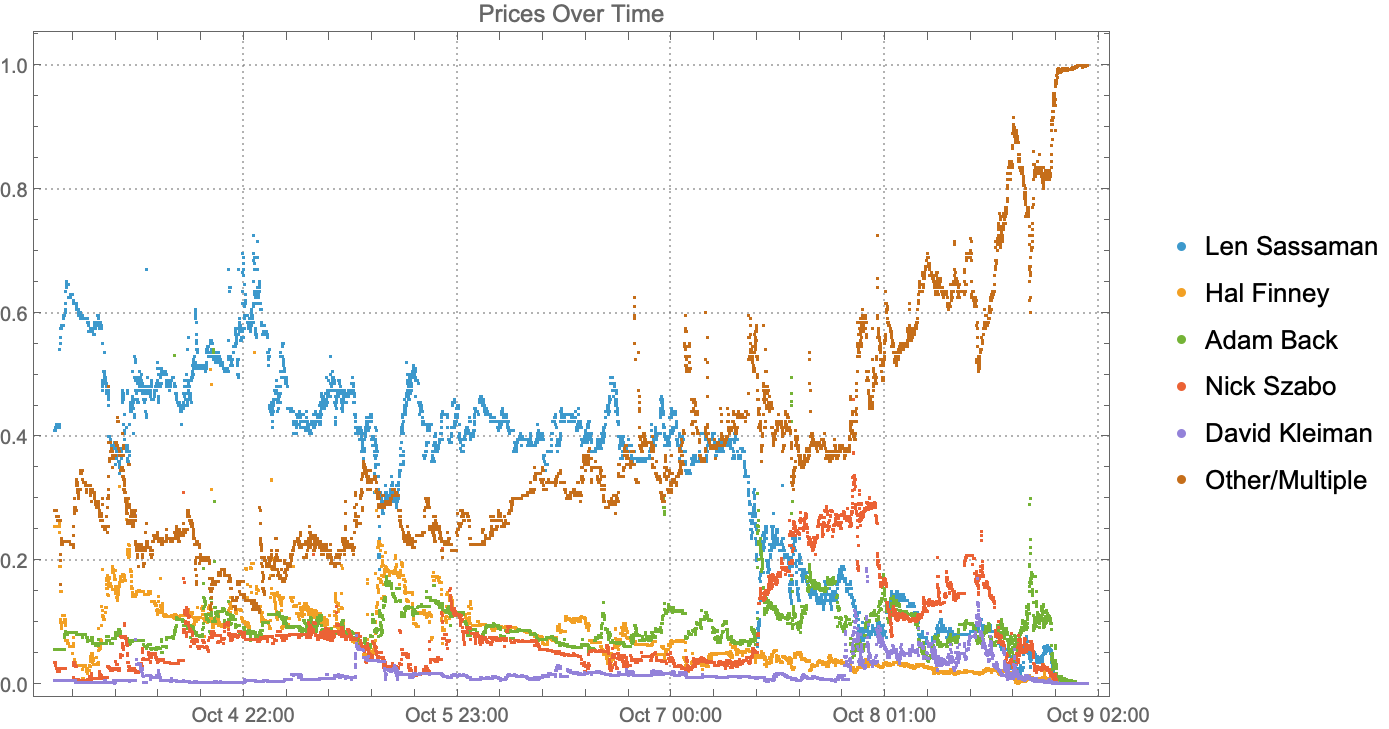
\includegraphics[width=\textwidth]{figures/graph.png}
  \caption{The price movements for 6 leading candidates in the Polymarket market for who would be named as Satoshi Nakamoto in the HBO documentary `Money Electric' which aired the evening of October 8.}
  \label{fig:example}
\end{figure}

\section{Example instantiation of formal definitions}
\label{app:example}

In section~\ref{sec:hbo}, we discussed an example market concerning who the HBO documentary `Money Electric' would name as Satoshi Nakamoto. In this section, we will see how this fits the definitions of a market, prediction market system, and the Arrow--Debreau special case. As discussed in Section~\ref{wf:mech}, Polymarket employs a market mechanism we call a yes/no bundle (YNB), as opposed to winner-take-all (WTA). YNB requires an extra step in the definitions so we will do a first pass with a simplified WTA submarket, and then add the full YNB market.

\subsection{Pass 1: Single WTA Market}

Consider a simplified market that questions whether one specific candidate, \eg Hal Finney, is named as Satoshi: yes or no. If through unforeseen circumstances, who the documentary names is not verifiable by the air date, the market resolves to no.

Recall Definition~\ref{def:market} of a market: 

\begin{definition}[Market]
A (single) market is a tuple $M=(E,\Omega,J,R)$, where $E$ is a well-defined uncertain event, $\Omega$ is a nonempty outcome space for $E$, $J$ is a finite index set of contract labels (“shares”), and $R=(R_j)_{j\in J}$ are nonnegative payoff functions with $R_j:\Omega\to\mathbb{R}_{\ge 0}$. 
We assume $|J|\ge|\Omega|$ and we require \emph{outcome distinguishability} on $\Omega$:
\[
\forall\,\omega\neq\omega'\in\Omega\ \ \exists\,j\in J:\ R_j(\omega)\neq R_j(\omega').
\]
When $M$ resolves to $\omega_M\in\Omega$, one unit of share $j\in J$ pays $R_j(\omega_M)$ (in units of $\mathcal{N}$ defined below).
\end{definition}

Event $E$ is whether or not Hal Finney is named as Satoshi in the documentary.

$\Omega$ is the set of resolution outcomes the market recognizes for $E$—the labels the system can publish at settlement. For this Hal-only binary market the outcome space is $\Omega=\{\mathsf{True},\mathsf{False}\}$. Here $\mathsf{True}$ means the documentary (per the market’s stated criteria) identifies Hal Finney as Satoshi; $\mathsf{False}$ aggregates all other possibilities (Hal not named, someone else named, no one named, the film does not air, or the identification is not verifiable by the resolution deadline).

%Once some $\omega\in\Omega$ is published, all payoffs $R_j(\omega)$ are determined.

We require that $\Omega$ contain no redundant labels. A label is redundant if it does not change at least one contract’s payoff: $\omega\sim\omega' \iff \forall j\in J,\ R_j(\omega)=R_j(\omega')$. For example, “Hal is named and it is raining’’ and “Hal is named and it is not raining’’ are distinct real-world states, but they cannot both appear in $\Omega$ since they both map to $\mathsf{True}$. The restriction can be written as:
\[
\forall\,\omega\neq\omega'\in\Omega\ \ \exists\,j\in J:\ R_j(\omega)\neq R_j(\omega').
\]

In a prediction market, there are a set of shares. If we label them and add them all to an index set, that set is $J$. For this example, $J=\{\textsf{YES},\textsf{NO}\}$: Hal Finney is named (yes) and else (no). This is a normal case where each share in $J$ corresponds to an outcome in $\Omega$ but it is possible that the number of shares could exceed the number of outcomes.\footnote{For example, consider a market of where Newcastle United (NUFC) finishes in the 2024-35 English Premier League season. Since there are 20 teams, the outcome has 20 possible labels: positions 1 to 20. Shares could exist for each of the 20 positions. But the outcome could also settle shares for whether NUFC finishes in the top 5 (which is relevant to champions league admittance), or shares on finishing in the bottom 3 (which is relevant to relegation).}

$J$ is the index set of contract labels—the names of the tradeable shares. In this binary market we take $J=\{\textsf{YES},\textsf{NO}\}$. 

The labels get their meaning from the component payoff functions $R_j:\Omega\to\mathbb{R}_{\ge 0}$. In this example, a payoff of 1 is given for shares that correctly predict the outcome and 0 otherwise. This means $R_{\textsf{YES}}(\mathsf{True})=1$, $R_{\textsf{YES}}(\mathsf{False})=0$, $R_{\textsf{NO}}(\mathsf{True})=0$, $R_{\textsf{NO}}(\mathsf{False})=1$.

Recall Definition~\ref{def:market} of a prediction--market system $\mathcal{S}=(\mathcal{M},\mathcal{N},\mathsf{Res})$:
$\mathcal{M}$ is the (countable) catalog of markets; $\mathcal{N}$ is the numeraire (unit of account used to price and settle claims);
and $\mathsf{Res}=\{\mathrm{res}_M\}_{M\in\mathcal{M}}$ assigns to each market $M$ a resolution register that is initially
$\bot$ and flips exactly once to some $\omega_M\in\Omega_M$.
When $\mathrm{res}_M\neq\bot$, we set $\omega_M:=\mathrm{res}_M$ and each unit of label $j\in J$ settles for $R_j(\omega_M)$ units of $\mathcal{N}$.

The market tuple $M=(E,\Omega,J,R)$ specifies \emph{what} to pay \emph{given} an outcome (via $R$).
The register $\mathrm{res}_M$ is the system’s single source of truth for \emph{which} outcome actually occurred:
before resolution $\mathrm{res}_M=\bot$ (no settlement), after resolution $\mathrm{res}_M=\omega_M\in\Omega_M$ (settlement applies).

Polymarket instantiates $\mathcal{S}$ with $\mathcal{M}$ equal to its live and historical markets, $\mathcal{N}$ the USD–denominated stablecoin USDC, and $\mathsf{Res}$ implemented by its on–chain resolution process (e.g., UMA’s optimistic oracle) that writes a single outcome to each $\mathrm{res}_M$.

For the Hal–only binary market, the system maintains a resolution register
$\mathrm{res}_{M_{\mathrm{Hal}}}\in\{\bot\}\cup\Omega$ with
$\Omega=\{\mathsf{True},\mathsf{False}\}$ (i.e., “yes/no” to the proposition).
The register is initially $\bot$ and, after the platform’s resolution process completes, the oracle writes a single value
$\omega_{M_{\mathrm{Hal}}}\in\Omega$ to the register.

Set $\omega_{M_{\mathrm{Hal}}}=\mathsf{True}$ iff the documentary (per stated criteria) identifies \emph{Hal Finney} as Satoshi; otherwise set $\omega_{M_{\mathrm{Hal}}}=\mathsf{False}$.

Shares are fully collateralized to \$1 in the numeraire $\mathcal{N}$ (USDC): a unit of \textsf{YES} pays $1$\,USDC at $\mathsf{True}$ and $0$\,USDC at $\mathsf{False}$; a unit of \textsf{NO} pays $1$\,USDC at $\mathsf{False}$ and $0$\,USDC at $\mathsf{True}$. Formally,
\[
R_{\textsf{YES}}(\mathsf{True})=1,\ \ R_{\textsf{YES}}(\mathsf{False})=0,\qquad
R_{\textsf{NO}}(\mathsf{True})=0,\ \ R_{\textsf{NO}}(\mathsf{False})=1.
\]

In the aired documentary, \emph{Peter Todd} was named; therefore
\[
\mathrm{res}_{M_{\mathrm{Hal}}}=\omega_{M_{\mathrm{Hal}}}=\mathsf{False},
\]
and each unit settles as
\[
\textsf{YES}\ \to\ 0\ \text{USDC},\qquad
\textsf{NO}\ \to\ 1\ \text{USDC}.
\]

% = = = 

This market is a winner--take--all (Arrow--Debreu) special case: there is a bijection $\iota:J\to\Omega$ and payoffs
$R_j(\omega)=\mathbf{1}\{\omega=\iota(j)\}$. Hence, for each $\omega\in\Omega$, exactly one label pays $1$ and all others pay $0$.
In the prediction--market system, the resolution register $\mathrm{res}_M\in\{\bot\}\cup\Omega$ is initially $\bot$ and flips exactly once to $\omega_M\in\Omega$; one unit of label $j\in J$ then settles for $R_j(\omega_M)$ units of the numeraire $\mathcal{N}$.

% = = = 

\subsection{Pass 2: YNB Market}

\paragraph{Families.}
Given an index set $C$, a \emph{family of markets} indexed by $C$ is a map $c\mapsto M_c$; we write $\{M_c\}_{c\in C}$. Each $c\in C$ names one market in the family.

\paragraph{Instantiation for the HBO event.}
Let $C$ be the set of candidates (e.g., $\{\textsf{Szabo},\textsf{Sassaman},\textsf{Back},\dots,\textsf{Other/Multiple}\}$).
Polymarket lists a family $\{M_c\}_{c\in C}$, one binary market per candidate:
\[
  M_c=(E_c,\Omega_c,J_c,R^{(c)}),\quad
  E_c=\text{``The documentary identifies $c$ as Satoshi''},\ 
  \Omega_c=\{\mathsf{True},\mathsf{False}\},\
  J_c=\{\textsf{YES},\textsf{NO}\},
\]
with indicator payoffs
\[
  R^{(c)}_{\textsf{YES}}(\mathsf{True})=1,\ R^{(c)}_{\textsf{YES}}(\mathsf{False})=0,\qquad
  R^{(c)}_{\textsf{NO}}(\mathsf{True})=0,\ R^{(c)}_{\textsf{NO}}(\mathsf{False})=1.
\]

\paragraph{System-level mapping to Polymarket.}
Polymarket instantiates the prediction–market system $\mathcal{S}=(\mathcal{M},\mathcal{N},\mathsf{Res})$ as follows:
\begin{itemize}
  \item $\mathcal{M}$ contains all candidate markets $\{M_c\}_{c\in C}$ under the HBO event (plus all other site markets).
  \item $\mathcal{N}$ is USDC (USD–denominated stablecoin). Each unit share settles to $0$ or $1$ USDC according to $R^{(c)}$.
  \item $\mathsf{Res}=\{\mathrm{res}_{M}\}_{M\in\mathcal{M}}$ gives each $M_c$ a register $\mathrm{res}_{M_c}\in\{\bot\}\cup\Omega_c$,
        initially $\bot$, that flips exactly once to $\omega_{M_c}\in\Omega_c$ when the platform’s oracle process (e.g., UMA’s optimistic oracle) writes the outcome on-chain.
\end{itemize}
Settlement in our notation is $R^{(c)}_j(\omega_{M_c})$ USDC for each unit of label $j\in J_c$.

\paragraph{What resolved in the HBO case.}
The documentary focused on \emph{Peter Todd}, which Polymarket grouped under \textsf{Other/Multiple}. Hence
\[
  \omega_{M_{\textsf{Other/Multiple}}}=\mathsf{True}
  \quad\text{and}\quad
  \omega_{M_c}=\mathsf{False}\ \text{ for all named }c\neq\textsf{Other/Multiple}.
\]
Equivalently: \textsf{Other/Multiple: YES} paid $1$ USDC; every named candidate’s \textsf{NO} paid $1$ USDC; the corresponding \textsf{YES} paid $0$ USDC.

\paragraph{Relation to Arrow--Debreu (single book) vs.\ Polymarket (bundle).}
A single winner–take–all (Arrow--Debreu) market would model the event as one market $M^\star=(E^\star,\Omega^\star,J^\star,R^\star)$ with
$\Omega^\star=C$ and $J^\star$ in bijection with $\Omega^\star$, so exactly one label pays $1$ at resolution.
Polymarket instead uses a \emph{bundle of binaries} $\{M_c\}_{c\in C}$ (one YES/NO pair per candidate). This is a different microstructure:
prices live in separate order books, and each market $M_c$ resolves independently via its own register $\mathrm{res}_{M_c}$.

\paragraph{Negative risk (Polymarket’s cross-market linkage).}
When the parent event is configured as \emph{negative risk}, Polymarket enables a conversion that links prices across the family:
informally, a \textsf{NO} on candidate $i$ is convertible into the basket of \textsf{YES} on all $j\neq i$.
At the price level this couples the binaries so that, up to frictions,
\[
\mathrm{price}(\textsf{NO}_i)\ \approx\ \sum_{j\neq i}\mathrm{price}(\textsf{YES}_j)
\quad\Longrightarrow\quad
\sum_{j\in C}\mathrm{price}(\textsf{YES}_j)\ \approx\ 1,
\]
making the bundle trade \emph{as if} it were a single Arrow--Debreu book while remaining, in our abstraction, a family $\{M_c\}$ with distinct $(E_c,\Omega_c,J_c,R^{(c)})$ and registers $\mathrm{res}_{M_c}$.
